%% Draft manuscript for Transportation Research Part B: Methodological (Elsevier).
%% Class: elsarticle, author-year (Harvard) references as required by the TR series.
%% Build: latexmk -pdf main.tex
\documentclass[preprint,12pt,authoryear]{elsarticle}

\usepackage[utf8]{inputenc}
\usepackage[T1]{fontenc}
\usepackage{amsmath,amssymb,amsthm,mathtools,bm}
\usepackage{booktabs,multirow,threeparttable}
\usepackage{graphicx}
\usepackage{enumitem}
\usepackage{xcolor}
\usepackage[colorlinks=true,citecolor=blue!60!black,linkcolor=blue!60!black,urlcolor=blue!60!black]{hyperref}
\usepackage{lineno}
\usepackage{setspace}
\usepackage[textsize=footnotesize,color=orange!25]{todonotes}

\linenumbers

%% Theorem-like environments
\newtheorem{proposition}{Proposition}
\newtheorem{corollary}{Corollary}
\theoremstyle{remark}
\newtheorem{remark}{Remark}

%% Notation
\newcommand{\NB}{\mathrm{NB}}
\newcommand{\PG}{\mathrm{PG}}
\newcommand{\CRT}{\mathrm{CRT}}
\newcommand{\Normal}{\mathrm{N}}
\newcommand{\Bern}{\mathrm{Bernoulli}}
\newcommand{\Betad}{\mathrm{Beta}}
\newcommand{\Gammad}{\mathrm{Gamma}}
\newcommand{\IG}{\mathrm{IG}}
\newcommand{\E}{\mathbb{E}}
\newcommand{\Var}{\operatorname{Var}}
\newcommand{\Cov}{\operatorname{Cov}}
\newcommand{\x}{\bm{x}}
\newcommand{\y}{\bm{y}}
\newcommand{\bbeta}{\bm{\beta}}
\newcommand{\bsigma}{\bm{\sigma}}
\newcommand{\bgamma}{\bm{\gamma}}
\newcommand{\bdelta}{\bm{\delta}}
\newcommand{\bomega}{\bm{\omega}}
\newcommand{\state}{S}
\newcommand{\tbd}[1]{\todo[inline,color=red!15]{#1}}
%% Rows of generated tables are read with the TeX primitive so they can sit inside tabular
\makeatletter
\newcommand{\tablerows}[1]{\@@input #1 }
\makeatother

\journal{Transportation Research Part B: Methodological}

\begin{document}

\begin{frontmatter}

\title{Which parameters should be random? Bayesian selection of fixed and random parameters in crash frequency models}

\author[inst1]{Ramakrushna Mishra\corref{cor1}}
\cortext[cor1]{Corresponding author.}
\ead{TBD@example.org}
\affiliation[inst1]{organization={TBD (affiliation)},
            city={TBD},
            country={India}}
%% \author[inst2]{Co-author}
%% \affiliation[inst2]{organization={},city={},country={}}

\begin{abstract}
Random parameters count models are a standard tool for representing unobserved heterogeneity in crash frequency analysis, yet which parameters are random is usually decided by testing one standard deviation at a time or by searching specifications with an information criterion. Inference is then reported conditional on one selected specification, and spurious heterogeneity is not controlled. This paper recasts the choice among excluded, fixed and random effects as Bayesian variable selection. A three-state spike-and-slab prior in a non-centered parameterization places point masses at zero on the mean and on the signed standard deviation of each candidate parameter, linked by a heredity structure. We show that in cross-sectional data a random parameter enters the count distribution only through a covariate-dependent lognormal variance, which adds a quadratic term to the conditional mean and makes overdispersion covariate dependent. Random parameters are therefore hard to separate from omitted curvature and varying dispersion unless panel data supply within-site covariance. A P\'olya-Gamma Gibbs sampler integrates out the site-specific draws when deciding whether a parameter is random.
{\color{red}[Simulation and application findings to be added.]}
The method reports, for every candidate, posterior probabilities of being excluded, fixed or random.
\end{abstract}

\begin{keyword}
Crash frequency \sep Random parameters \sep Unobserved heterogeneity \sep Bayesian variable selection \sep Spike-and-slab prior \sep P\'olya-Gamma augmentation
\end{keyword}

\end{frontmatter}

\onehalfspacing

\section{Introduction}\label{sec:intro}

Crash frequency models relate the number of crashes on a roadway entity over a period of time to traffic exposure, geometric design and environmental conditions. They underpin safety performance functions, network screening and the evaluation of countermeasures \citep{lord2010statistical}. Over the past fifteen years, models with random parameters have become the standard way to accommodate unobserved heterogeneity, the fact that the effect of a measured factor varies across sites because of conditions that are not measured \citep{anastasopoulos2009note, mannering2014analytic, mannering2016unobserved}. In a random parameters negative binomial (RPNB) model the coefficient of a covariate is allowed to vary across sites according to a distribution, usually normal, whose mean and standard deviation are estimated from the data, either by simulated maximum likelihood \citep{train2009discrete, bhat2003simulation} or by Markov chain Monte Carlo \citep{elbasyouny2009accident, buddhavarapu2016modeling}.

The flexibility comes with a decision that receives far less attention than the estimation itself: the analyst must choose which coefficients are random. With $p$ candidate covariates, each of which may be excluded, enter with a fixed coefficient, or enter with a random coefficient, there are $3^p$ candidate specifications before heterogeneity in means, heterogeneity in variances or correlation among random parameters is considered. In practice the decision is made sequentially. Covariates are screened in a fixed parameters model, each surviving coefficient is then tried as random, and a random parameter is kept when its estimated standard deviation is statistically significant and fixed otherwise \citep[e.g.,][]{zeng2017multivariate}. More recent work searches the specification space with metaheuristics that minimize an information criterion \citep{ahern2024extensive}. Both strategies settle on a single specification and then report standard errors, marginal effects and policy implications conditional on it, as though it had been fixed before the data were seen.

This practice has three consequences. First, specification uncertainty is not reported, even though it can be large when heterogeneity is modest relative to the Poisson and gamma noise in crash counts. Second, because many standard deviations are tested, often in an order chosen by the analyst, the probability of declaring at least one spurious random parameter grows with the number of candidates and is not controlled. Third, as we show in Section~\ref{sec:identification}, a normally distributed random parameter changes the distribution of counts through a covariate-dependent variance of a lognormal error. That variance adds a quadratic term to the conditional mean and makes overdispersion depend on the covariate, so a detected random parameter may reflect an omitted nonlinear effect or a covariate-dependent dispersion as much as genuine heterogeneity in the effect. Panel data contain information that separates these explanations, but our simulations show that a misspecified model does not use it.

This paper treats the specification of a random parameters model as a variable selection problem and solves it inside a single Bayesian model. Each candidate covariate is assigned one of three states, excluded, fixed or random, and the posterior distribution over these states is computed jointly with the model parameters. The contributions are as follows.
\begin{enumerate}[label=(\roman*),leftmargin=*]
\item \emph{A three-state spike-and-slab prior for effect structure.} Writing the random parameter in non-centered form, $\beta_{ij}=\beta_j+\sigma_j z_{ij}$ with $z_{ij}\sim\Normal(0,1)$ and $\sigma_j$ allowed to take either sign, turns the question ``is this parameter random?'' into the question ``is $\sigma_j$ zero?'', which has the same form as the question ``is $\beta_j$ zero?'' \citep{fruhwirth2010stochastic}. Point-mass spikes on $\beta_j$ and $\sigma_j$, linked by a heredity prior and given beta-binomial hyperpriors, produce posterior probabilities for the three states with an automatic adjustment for the number of candidates \citep{scott2010bayes}.
\item \emph{Identification results that matter for practice.} We characterize how random parameters enter the distribution of crash counts in cross-sectional and panel data, show that the random parameter variance is confounded with the fixed effect for binary covariates and with curvature for continuous covariates, and show that within-site covariance in panel data identifies random parameters separately from the negative binomial dispersion. We then show by simulation that this information is not enough when the mean or the dispersion is misspecified, which motivates selecting the mean curvature and the dispersion covariates jointly with the random parameters.
\item \emph{An efficient sampler.} P\'olya-Gamma augmentation \citep{polson2013bayesian} and the Chinese restaurant table augmentation for the negative binomial dispersion \citep{zhou2015negative} make all regression updates conditionally Gaussian. The step that decides whether a parameter is random integrates out the site-specific draws $z_{ij}$, which reduces it to a one-dimensional integral with a closed-form integrand. Without this step the sampler rarely switches a random parameter on, because a freshly drawn $z_{ij}$ carries no information about the data.
\item \emph{Evidence.} In a simulation study with 100 replications per design, the method recovers the full specification in 60\% of replications with 1{,}000 sites observed over five periods, against 1\% for the sequential procedure, none for its Bayesian counterpart based on the deviance information criterion and 37\% for an information criterion search, and its intervals for the random-parameter standard deviations cover the truth far more often. A false discovery rate rule trades detection for control of false claims of heterogeneity. Omitted curvature and covariate-dependent dispersion produce spurious random parameters under every method that holds the mean linear and the dispersion constant. Squared covariates as fixed-only candidates remove the first. Spike-and-slab selection of dispersion covariates, updated by reversible jump, removes the second in panel data (spurious random parameters in 1\% of replications against 90\% or more) and reduces it from over 90\% to 35\% in cross-sectional data, at little cost when the dispersion is in fact constant. \tbd{Application (Section~\ref{sec:application}).}
\end{enumerate}

The remainder of the paper is organized as follows. Section~\ref{sec:background} reviews random parameters crash models and Bayesian variable selection. Section~\ref{sec:model} presents the model, the identification results and the prior. Section~\ref{sec:computation} develops the sampler. Section~\ref{sec:simulation} reports a simulation study and Section~\ref{sec:application} an application to \tbd{data set}. Section~\ref{sec:discussion} discusses extensions and limitations and Section~\ref{sec:conclusion} concludes. Proofs and derivations are collected in the appendices.

\section{Background}\label{sec:background}

\subsection{Random parameters in crash frequency analysis}

Crash counts are overdispersed relative to the Poisson distribution, and the negative binomial (NB) model, which mixes the Poisson rate over a gamma distribution, has long been the default for safety performance functions \citep{lord2010statistical}. Fixed parameters NB models assume that a covariate has the same effect at every site. Random parameters models relax this by letting coefficients vary across observations, which captures heterogeneity due to unobserved driver, vehicle, roadway and environmental factors \citep{mannering2016unobserved}. Following \citet{anastasopoulos2009note} and \citet{milton2008highway}, random parameters count and discrete outcome models have been applied to segment and intersection crash frequencies, crash rates and injury severities, often with extensions to heterogeneity in means and variances, correlated random parameters and temporal instability \citep{mannering2014analytic, mannering2018temporal}. Estimation is typically by simulated maximum likelihood with Halton draws \citep{bhat2003simulation, train2009discrete} or by full Bayesian methods \citep{elbasyouny2009accident}. \citet{buddhavarapu2016modeling} used P\'olya-Gamma augmentation to estimate finite mixture random parameters models for spatially correlated crash counts, which shows that the computational route used in this paper is practical for safety data.

\subsection{How specifications are chosen}

Textbook treatments describe a sequential procedure \citep{washington2020statistical}. Candidate covariates are first screened in a fixed parameters model. Each retained coefficient is then specified as random, and the random specification is kept when the standard deviation of the parameter distribution is statistically different from zero, otherwise the parameter is treated as fixed. In Bayesian applications the same decision is made by inspecting a credible interval for the standard deviation, or by comparing deviance information criteria of models with and without the random parameter \citep[e.g.,][]{zeng2017multivariate}. Because the number of candidate specifications grows as $3^p$, and faster once heterogeneity in means or correlation among random parameters is allowed, \citet{ahern2024extensive} formulated specification search as a combinatorial optimization problem and solved it with metaheuristics that minimize the Bayesian information criterion.

These procedures share two features. They return one specification, so the uncertainty about which parameters are random is not propagated into estimates of marginal effects or into decisions based on them. They also perform many tests of variance components, a setting in which classical tests are non-standard because the null value $\sigma_j=0$ lies on the boundary of the parameter space, and in which no adjustment is made for the number of tests.

\subsection{Bayesian variable selection and selection of random effects}

Spike-and-slab priors place a mixture of a point mass (or a narrow distribution) at zero and a diffuse distribution on each regression coefficient, so that the posterior probability of the slab component measures the evidence that a variable belongs in the model \citep{mitchell1988bayesian, george1993variable, ishwaran2005spike}. Treating the prior inclusion probability as unknown, with a beta hyperprior, yields an automatic multiplicity adjustment \citep{scott2010bayes}, and the median probability model is optimal for prediction under conditions given by \citet{barbieri2004optimal}. Continuous shrinkage alternatives include the Bayesian lasso \citep{park2008bayesian, kyung2010penalized}, the horseshoe \citep{carvalho2010horseshoe} and the spike-and-slab lasso \citep{rockova2018spike}. \citet{ohara2009review} compare several of these methods in practice.

Selecting random effects is harder than selecting fixed effects because a variance cannot be negative, so a spike at zero sits on the boundary of the parameter space. \citet{chen2003random} and \citet{kinney2007fixed} selected random effects in linear and logistic mixed models by reparameterizing the covariance matrix of the random effects. \citet{fruhwirth2008bayesian} and \citet{fruhwirth2010stochastic} introduced the device that we adopt: write the random component as $\sigma_j z_{ij}$ with $\sigma_j\in\mathbb{R}$, so that $\sigma_j$ enters the linear predictor linearly given $z_{ij}$ and can receive an ordinary spike-and-slab prior. A Gaussian slab on the signed $\sigma_j$ implies a scaled $\chi^2_1$ prior on the variance $\sigma_j^2$, which has substantial mass near zero. Inverse-gamma priors on variances, by contrast, have vanishing density at zero and can overstate heterogeneity when the data are weakly informative \citep{gelman2006prior}. \citet{bitto2019achieving} extended the idea to continuous shrinkage in time-varying parameter models.

Deciding jointly whether a coefficient enters and whether it varies is a bi-level selection problem in which the mean and the standard deviation of a parameter form a natural group. Bi-level and group spike-and-slab priors have been studied for linear regression \citep{xu2015bayesian, yang2020consistent, bai2022spike}, and heredity priors that let the inclusion of one term depend on another go back to \citet{chipman1996bayesian}. To our knowledge these tools have not been brought together for the specification of random parameters crash models, where the groups have a specific structure (a mean and a standard deviation), the likelihood is negative binomial, and the random components are observation specific rather than shared within clusters. \tbd{Confirm with a final literature check before submission, including recent AMAR, AA\&P and TR-B issues.}

\section{Model}\label{sec:model}

\subsection{Random parameters negative binomial model}\label{sec:rpnb}

Let $y_{it}$ be the number of crashes at site $i=1,\dots,n$ in period $t=1,\dots,T_i$, with $N=\sum_i T_i$ observations in total. Cross-sectional data correspond to $T_i=1$. Let $\x_{it}=(x_{it1},\dots,x_{itp})^\top$ collect $p$ candidate covariates and let $o_{it}$ be a known offset, for example the logarithm of segment length times the length of the period. Conditional on a rate $\lambda_{it}$, the count follows a negative binomial distribution with mean $\lambda_{it}$ and dispersion $r>0$,
\begin{equation}\label{eq:nb}
\Pr(y_{it}=y \mid \lambda_{it}, r)=\frac{\Gamma(y+r)}{\Gamma(r)\,y!}\left(\frac{r}{r+\lambda_{it}}\right)^{r}\left(\frac{\lambda_{it}}{r+\lambda_{it}}\right)^{y},
\end{equation}
so that $\Var(y_{it}\mid\lambda_{it})=\lambda_{it}+\lambda_{it}^2/r$.
The random parameters specification is
\begin{equation}\label{eq:rp}
\log\lambda_{it}=o_{it}+\alpha+\sum_{j=1}^{p}x_{itj}\,\beta_{ij},
\qquad \beta_{ij}=\beta_j+\sigma_j z_{ij},
\qquad z_{ij}\overset{\text{iid}}{\sim}\Normal(0,1),
\end{equation}
so that the coefficient of covariate $j$ at site $i$ is normally distributed with mean $\beta_j$ and standard deviation $|\sigma_j|$. The draw $z_{ij}$ is shared by all periods of site $i$, so in panel data a site keeps its coefficient over time, while in cross-sectional data each observation has its own coefficient. Substituting the second equation into the first gives the non-centered form
\begin{equation}\label{eq:noncentered}
\log\lambda_{it}=o_{it}+\alpha+\x_{it}^\top\bbeta+\varepsilon_{it},
\qquad \varepsilon_{it}=\sum_{j=1}^{p}\sigma_j\,x_{itj}\,z_{ij}.
\end{equation}
We allow $\sigma_j$ to take any real value. Its sign is not identified, because $(\sigma_j,z_{ij})$ and $(-\sigma_j,-z_{ij})$ give the same likelihood, and all reported quantities depend on $\sigma_j$ only through $|\sigma_j|$. The advantage of \eqref{eq:noncentered} is that, given $z_{ij}$, the parameter $\sigma_j$ enters the linear predictor linearly, exactly as $\beta_j$ does \citep{papaspiliopoulos2007general, fruhwirth2010stochastic}.

Each covariate is in one of three states,
\begin{equation}\label{eq:states}
\state_j=\begin{cases}
\mathrm{E}\ (\text{excluded}) & \text{if } \beta_j=0 \text{ and } \sigma_j=0,\\
\mathrm{F}\ (\text{fixed}) & \text{if } \beta_j\neq 0 \text{ and } \sigma_j=0,\\
\mathrm{R}\ (\text{random}) & \text{if } \sigma_j\neq 0 .
\end{cases}
\end{equation}
The specification problem is to learn $\state=(\state_1,\dots,\state_p)$. Some columns of $\x_{it}$ may be admissible only as fixed effects, for example quadratic terms introduced to protect against the confounding described in Section~\ref{sec:identification}. For those columns we set $\sigma_j=0$.

\begin{remark}[Centering changes the model]\label{rem:centering}
For a fixed parameter, replacing $x_{itj}$ by $x_{itj}-c$ only shifts the intercept. For a random parameter it does more: $\beta_{ij}(x_{itj}-c)=\beta_{ij}x_{itj}-c\beta_j-c\sigma_j z_{ij}$, and the last term is a site-specific random intercept. Centering therefore moves heterogeneity between the slope and the intercept and changes the variance function $v(\cdot)$ defined below. We scale continuous covariates by their standard deviations but do not center them, and we leave binary covariates coded $0/1$, which keeps the conventional interpretation of random parameters.
\end{remark}

\subsection{What crash data can reveal about random parameters}\label{sec:identification}

Write $\eta_{it}=o_{it}+\alpha+\x_{it}^\top\bbeta$, $D=\operatorname{diag}(\sigma_1^2,\dots,\sigma_p^2)$ and $v(\x)=\x^\top D\x=\sum_j\sigma_j^2x_j^2$. Given the covariates, $\varepsilon_{it}$ in \eqref{eq:noncentered} is a sum of independent normal terms, so $\varepsilon_{it}\sim\Normal\{0,v(\x_{it})\}$ and $\Cov(\varepsilon_{it},\varepsilon_{is})=\x_{it}^\top D\,\x_{is}$. The following results, proved in \ref{app:proofs}, describe what this implies for the distribution of crash counts.

\begin{proposition}[Cross-sectional data]\label{prop:cross}
Let $T_i=1$ and drop the index $t$. Then:
\begin{enumerate}[label=(\alph*)]
\item The likelihood contribution of site $i$ is
\[
\int \NB\{y_i \mid e^{\eta_i+u}, r\}\,\phi\{u \mid 0, v(\x_i)\}\,du,
\]
where $\phi(\cdot\mid 0,v)$ is the normal density with variance $v$. The likelihood therefore depends on $(\sigma_1,\dots,\sigma_p)$ only through the variance function $v(\cdot)$.
\item The conditional mean and variance are
\begin{equation}\label{eq:moments}
\begin{aligned}
\mu_i&=\E(y_i\mid\x_i)=\exp\{\eta_i+v(\x_i)/2\},\\
\Var(y_i\mid\x_i)&=\mu_i+\mu_i^2\left\{\left(1+\tfrac{1}{r}\right)e^{v(\x_i)}-1\right\}.
\end{aligned}
\end{equation}
\item A necessary condition for $(\sigma_1^2,\dots,\sigma_p^2)$ to be locally identified at a point with all $\sigma_j^2>0$ is that the functions $\x\mapsto x_j^2$, $j=1,\dots,p$, be linearly independent on the support of $\x$.
\end{enumerate}
\end{proposition}

Part (b) has three consequences that bear directly on specification practice.

\begin{corollary}\label{cor:confounding}
Under the conditions of Proposition~\ref{prop:cross}:
\begin{enumerate}[label=(\roman*)]
\item If $x_j$ is binary, then $x_j^2=x_j$ and the log mean contains $x_j(\beta_j+\sigma_j^2/2)$. The mean identifies only $\beta_j+\sigma_j^2/2$, and information about $\sigma_j$ comes solely from the difference in overdispersion between sites with $x_j=1$ and $x_j=0$.
\item If $x_j$ is continuous, a random parameter adds $\sigma_j^2x_j^2/2$ to the log mean, which is indistinguishable in the mean from a fixed quadratic effect with a positive coefficient. A convex effect omitted from a linear specification can therefore surface as a spurious random parameter. A concave effect cannot.
\item The first two conditional moments in \eqref{eq:moments} coincide with those of a fixed parameters NB model with log mean $\eta_i+v(\x_i)/2$ and covariate-dependent dispersion $r(\x_i)=\left[(1+1/r)e^{v(\x_i)}-1\right]^{-1}$. Separating a random parameter from varying dispersion \citep{miaou2003modeling} therefore relies on higher moments, that is, on the difference between lognormal and gamma mixing.
\end{enumerate}
\end{corollary}

Panel data change the picture because the same draw $z_{ij}$ affects all periods of a site.

\begin{proposition}[Panel data]\label{prop:panel}
For $t\neq s$,
\begin{equation}\label{eq:panelcov}
\Cov(y_{it},y_{is}\mid \x_{i1},\dots,\x_{iT_i})=\mu_{it}\,\mu_{is}\left\{\exp\left(\x_{it}^\top D\,\x_{is}\right)-1\right\},
\end{equation}
where $\mu_{it}=\exp\{\eta_{it}+v(\x_{it})/2\}$. The covariance does not depend on the dispersion $r$.
\end{proposition}

The negative binomial dispersion, fixed or covariate dependent, acts independently in each period and implies zero within-site covariance. The covariance in \eqref{eq:panelcov} is therefore information about $D$ that the dispersion cannot mimic. A site-level random intercept, which corresponds to a column $x_{it0}\equiv 1$, also induces within-site covariance, but a constant one. Random slopes are identified from how the covariance changes with the covariates, which is why the random intercept should be included among the candidates in panel applications.

Proposition~\ref{prop:panel} is derived under a correctly specified model. It shows that the within-site covariance carries information about $D$ that the dispersion cannot mimic, but a misspecified model need not use that information well, and two failures matter in practice. First, suppose the mean omits a term $g(x_{ij})$ in a covariate that is constant within a site, as geometric variables usually are. The omitted term is then the same in every period of site $i$, and the random component $\sigma_jx_{ij}z_{ij}$, whose draw is also shared across periods, can absorb it by setting $z_{ij}\approx g(x_{ij})/(\sigma_jx_{ij})$. Second, suppose the dispersion varies with a covariate but the model assumes a common $r$. By Proposition~\ref{prop:cross}(b), a random parameter on that covariate raises the marginal variance at the sites where the data are more dispersed, and the gain in fit can outweigh the cost of implying a within-site covariance that the data do not show. Section~\ref{sec:sim-bc} shows that both failures occur in panel data as well as in cross-sectional data.

\begin{remark}[Practical implications]\label{rem:practice}
Evidence for a random parameter is evidence of a covariate-dependent variance in the log rate. Genuine heterogeneity in the effect can produce it, but so can omitted convex curvature and varying dispersion, and panel data do not remove either confounder when the model is misspecified. We therefore include quadratic terms of continuous covariates as fixed-only candidates in cross-sectional and panel applications alike, so that curvature is not absorbed into $\sigma_j$. Varying dispersion calls for the analogous safeguard on the dispersion side, which is to model the dispersion with its own candidates, as in \eqref{eq:dispersion} below. Without it, a selected random parameter should be read as evidence of heterogeneity in either the effect or the dispersion.
\end{remark}

\subsection{Prior specification}\label{sec:prior}

We introduce indicators $\gamma_j=\mathbb{1}(\beta_j\neq0)$ and $\delta_j=\mathbb{1}(\sigma_j\neq0)$ and use point-mass spike-and-slab priors for both:
\begin{align}
\beta_j\mid\gamma_j,\tau_\beta &\sim \gamma_j\,\Normal(0,\tau_\beta^2)+(1-\gamma_j)\,\mathbb{1}_{\{0\}}, \label{eq:prior-beta}\\
\gamma_j\mid\pi_\beta &\sim \Bern(\pi_\beta), \nonumber\\
\sigma_j\mid\delta_j,\tau_\sigma &\sim \delta_j\,\Normal(0,\tau_\sigma^2)+(1-\delta_j)\,\mathbb{1}_{\{0\}}, \label{eq:prior-sigma}\\
\delta_j\mid\gamma_j,\pi_{\sigma1},\pi_{\sigma0} &\sim \Bern\{\gamma_j\pi_{\sigma1}+(1-\gamma_j)\pi_{\sigma0}\}. \nonumber
\end{align}
The prior for $\delta_j$ encodes heredity \citep{chipman1996bayesian}. Under \emph{strong heredity}, $\pi_{\sigma0}=0$ and a parameter can be random only if its mean is nonzero, which matches the way specifications are built in practice. Under \emph{weak heredity}, $\pi_{\sigma0}$ is small but positive, which admits effects whose mean is zero but whose sign varies across sites. The three states in \eqref{eq:states} correspond to $(\gamma_j,\delta_j)=(0,0)$, $(1,0)$ and $\delta_j=1$.

The inclusion probabilities receive beta hyperpriors, $\pi_\beta\sim\Betad(a_\beta,b_\beta)$, $\pi_{\sigma1}\sim\Betad(a_\sigma,b_\sigma)$ and, under weak heredity, $\pi_{\sigma0}\sim\Betad(a_0,b_0)$. Learning these probabilities from the data produces the multiplicity adjustment of \citet{scott2010bayes}: as more candidates are considered, the prior probability that any particular one is random falls in line with the evidence that most are not. The slab scales $\tau_\beta$ and $\tau_\sigma$ are fixed at substantive values rather than learned. When the slab scale and the inclusion probability are both learned, a posterior with many coefficients in a narrow slab and a posterior with few coefficients in a wide slab fit the data almost equally well, and in small samples the sampler drifts toward the first, including nearly every candidate. We observed exactly this behavior in pilot runs with half-Cauchy priors on the slab scales, which we therefore retain only as a sensitivity option (Section~\ref{sec:computation}). A Gaussian slab on the signed $\sigma_j$ implies $\sigma_j^2\mid\delta_j=1\sim\tau_\sigma^2\chi^2_1$, a prior on the random parameter variance that places substantial mass near zero. Vague inverse-gamma priors on variances, common in applied Bayesian crash modeling, have vanishing density at zero and tend to overstate heterogeneity when the data are weak \citep{gelman2006prior}. Finally, $\alpha\sim\Normal(0,s_\alpha^2)$ and $r\sim\Gammad(a_r,b_r)$.

\paragraph{Default hyperparameters} With covariates scaled to unit standard deviation we use $a_\beta=b_\beta=a_\sigma=b_\sigma=1$, $\tau_\beta=\tau_\sigma=0.5$, $s_\alpha=10$, $a_r=1$ and $b_r=0.1$. A slab standard deviation of $0.5$ for $\beta_j$ makes rate ratios between about $0.37$ and $2.7$ per standard deviation of a covariate plausible, which covers the effects reported in safety performance functions. With $|\sigma_j|=0.5$, the rate ratio for a one-standard-deviation increase in $x_j$ at a site one standard deviation above or below the average effect differs from the average rate ratio by a factor of $e^{\pm0.5}$, about $0.61$ to $1.65$, which is already substantial heterogeneity, so $\tau_\sigma=0.5$ makes such values typical without ruling out larger ones. \tbd{Sensitivity analysis to $(a_\sigma,b_\sigma)$, $\tau_\sigma$ and heredity in Sections~\ref{sec:simulation} and~\ref{sec:application}.}

\paragraph{Covariate-dependent dispersion} Section~\ref{sec:sim-bc} shows that a dispersion that varies with a covariate is mistaken for a random parameter on that covariate unless the dispersion itself is modeled. The full version of the method therefore lets the dispersion depend on candidate covariates $\bm w_{it}$, which in our experiments are the same as the candidates for the mean:
\begin{equation}\label{eq:dispersion}
\begin{gathered}
\log r_{it}=\rho_0+\bm w_{it}^\top\bm\rho,\\
\rho_k\mid\eta_k\sim\eta_k\,\Normal(0,\tau_\rho^2)+(1-\eta_k)\,\mathbb{1}_{\{0\}},\qquad
\eta_k\mid\pi_\rho\sim\Bern(\pi_\rho),
\end{gathered}
\end{equation}
with $\pi_\rho\sim\Betad(1,1)$, $\tau_\rho=0.5$ and $\rho_0\sim\Normal(0,2^2)$. The dispersion is bounded below, $r_{it}=\max\{\exp(\rho_0+\bm w_{it}^\top\bm\rho),\,0.01\}$, which allows a variance of up to $\mu+100\mu^2$, far beyond what crash data show, and keeps the P\'olya-Gamma draws of Section~\ref{sec:computation} well defined. Extra variation linked to a covariate then has three competing explanations within one model: a random parameter on the covariate, a dispersion effect of the covariate and, through the squared candidates, curvature in the mean. The posterior weighs them against each other, and a candidate is declared to have a dispersion effect if $\Pr(\eta_k=1\mid\y)>1/2$.

\subsection{Posterior summaries for practice}\label{sec:summaries}

For each candidate the sampler returns the posterior state probabilities
\begin{equation}\label{eq:stateprob}
\begin{aligned}
P_j(\mathrm{E})&=\Pr(\gamma_j=0,\delta_j=0\mid\y),\\
P_j(\mathrm{F})&=\Pr(\gamma_j=1,\delta_j=0\mid\y),\\
P_j(\mathrm{R})&=\Pr(\delta_j=1\mid\y).
\end{aligned}
\end{equation}
Our default decision applies the median probability rule of \citet{barbieri2004optimal} to each indicator: a candidate is declared random if $P_j(\mathrm{R})>1/2$, and otherwise fixed if $\Pr(\gamma_j=1\mid\y)>1/2$. Under a zero-one loss for each covariate the Bayes decision would instead be the state with the largest posterior probability. In the simulation study of Section~\ref{sec:simulation} the two rules disagreed for about 3\% of candidates. When the claim of interest is that a parameter is random, the set $\widehat{\mathcal R}_c=\{j:P_j(\mathrm{R})\ge c\}$ has estimated Bayesian false discovery rate $\sum_{j\in\widehat{\mathcal R}_c}\{1-P_j(\mathrm{R})\}/|\widehat{\mathcal R}_c|$, and $c$ can be chosen as the smallest threshold that keeps this rate below a target $q$ \citep{newton2004detecting}. Effect summaries are averaged over specifications: the posterior distributions of $\beta_j$ and $|\sigma_j|$, the share of sites with a positive effect $\Phi(\beta_j/|\sigma_j|)$ for parameters in state R, and site-specific coefficients $\beta_{ij}$, which are shrunk toward $\beta_j$ according to the information in each site's data.

\section{Posterior computation}\label{sec:computation}

\subsection{Augmentation}

Write the negative binomial in terms of its log odds. Let $\lambda_{it}=r\,e^{\psi_{it}}$ with
\begin{equation}\label{eq:psi}
\psi_{it}=o_{it}+\alpha+\x_{it}^\top\bbeta+\varepsilon_{it},
\end{equation}
so that the intercept $\alpha$ is on the log-odds scale and the intercept of the mean model is $\alpha+\log r$. The slopes $\bbeta$ and the random components $\varepsilon_{it}$ are unchanged. In this parameterization \eqref{eq:nb} becomes
\begin{equation}\label{eq:nb-logit}
\Pr(y_{it}\mid\psi_{it},r)=\frac{\Gamma(y_{it}+r)}{\Gamma(r)\,y_{it}!}\,\frac{\left(e^{\psi_{it}}\right)^{y_{it}}}{\left(1+e^{\psi_{it}}\right)^{y_{it}+r}} .
\end{equation}
By the P\'olya-Gamma identity of \citet{polson2013bayesian},
\begin{equation}\label{eq:pg}
\frac{\left(e^{\psi}\right)^{y}}{\left(1+e^{\psi}\right)^{y+r}}
=2^{-(y+r)}\,e^{\kappa\psi}\int_0^\infty e^{-\omega\psi^2/2}\,p_{\PG}(\omega\mid y+r,0)\,d\omega,
\qquad \kappa=\frac{y-r}{2},
\end{equation}
where $p_{\PG}(\cdot\mid b,0)$ is the P\'olya-Gamma density. Conditional on $\omega_{it}$, the likelihood in $\psi_{it}$ is proportional to $\exp\{-\omega_{it}(\tilde y_{it}-\psi_{it})^2/2\}$ with working response $\tilde y_{it}=\kappa_{it}/\omega_{it}$. Every coefficient that enters $\psi_{it}$ linearly therefore has a Gaussian conditional likelihood, which is what makes the spike-and-slab updates below available in closed form. For the dispersion we use the Chinese restaurant table (CRT) augmentation \citep{zhou2012lognormal, zhou2015negative}: if $L_{it}\mid y_{it},r\sim\CRT(y_{it},r)$, that is $L_{it}=\sum_{l=1}^{y_{it}}b_l$ with independent $b_l\sim\Bern\{r/(r+l-1)\}$, then a gamma prior on $r$ is conjugate.

\subsection{Why the random draws must be integrated out}\label{sec:collapse}

A direct Gibbs sampler would update $(\delta_j,\sigma_j)$ given the current draws $z_{1j},\dots,z_{nj}$. When $\delta_j=0$ these draws do not enter the likelihood, so their full conditional is the prior and they are pure noise. The evidence for switching the parameter on is then computed with a vector of $n$ random numbers that bears no relation to the data, and with realistic $n$ the probability of a switch is negligible. The sampler would rarely, if ever, discover a random parameter it did not start with. We avoid this by updating the block $(\delta_j,\sigma_j,z_{1j},\dots,z_{nj})$ jointly: first $(\delta_j,\sigma_j)$ from their conditional distribution with the $z_{ij}$ integrated out, then the $z_{ij}$ given $(\delta_j,\sigma_j)$. Because the integral over $z_{ij}$ is Gaussian, the marginal evidence has a closed-form integrand, as the next result shows (derivation in \ref{app:derivations}).

\begin{proposition}[Marginal evidence for a random parameter]\label{prop:marginal}
Fix all quantities except $(\sigma_j,z_{1j},\dots,z_{nj})$ and let $e_{it}=\tilde y_{it}-(\psi_{it}-\sigma_j x_{itj}z_{ij})$ be the working residual that excludes the contribution of the $j$th random component. Define the site-level statistics
\[
q_{ij}=\sum_{t=1}^{T_i}\omega_{it}x_{itj}^2,\qquad b_{ij}=\sum_{t=1}^{T_i}\omega_{it}x_{itj}e_{it}.
\]
Then, with $z_{ij}\sim\Normal(0,1)$ integrated out, the ratio of the conditional likelihood at $\sigma_j=\sigma$ to that at $\sigma_j=0$ is $\exp\{\ell_j(\sigma)\}$, where
\begin{equation}\label{eq:ell}
\ell_j(\sigma)=\sum_{i=1}^{n}\left\{-\frac12\log\left(1+\sigma^2q_{ij}\right)+\frac{\sigma^2b_{ij}^2}{2\left(1+\sigma^2q_{ij}\right)}\right\}.
\end{equation}
Given $\sigma_j=\sigma$, the draws are conditionally independent with
\[
z_{ij}\sim\Normal\left(\frac{\sigma b_{ij}}{1+\sigma^2q_{ij}},\ \frac{1}{1+\sigma^2q_{ij}}\right).
\]
\end{proposition}

The Bayes factor for a random parameter,
\begin{equation}\label{eq:bf-sigma}
\mathrm{BF}^{\sigma}_j=\int_{-\infty}^{\infty}\exp\{\ell_j(\sigma)\}\,\phi(\sigma\mid0,\tau_\sigma^2)\,d\sigma,
\end{equation}
is a one-dimensional integral of a smooth function that is symmetric in $\sigma$, so it is computed accurately on a grid over $\sigma\ge0$. Each evaluation of $\ell_j$ costs $O(n)$ operations once $q_{ij}$ and $b_{ij}$ are formed. The analogous Bayes factor for a fixed effect is available in closed form,
\begin{equation}\label{eq:bf-beta}
\mathrm{BF}^{\beta}_j=\left(1+\tau_\beta^2S_j\right)^{-1/2}\exp\left\{\frac{B_j^2}{2\left(S_j+\tau_\beta^{-2}\right)}\right\},
\end{equation}
where $S_j=\sum_{i,t}\omega_{it}x_{itj}^2$, $B_j=\sum_{i,t}\omega_{it}x_{itj}e^{\beta}_{it}$ and $e^{\beta}_{it}=\tilde y_{it}-(\psi_{it}-x_{itj}\beta_j)$.

\subsection{The sampler}

One sweep of the sampler is summarized in Box~1. Steps 1 and 5 are blocked updates in which some variables are integrated out and then redrawn immediately, which preserves the target distribution \citep{vandyk2008partially}. All draws are exact except that of $|\sigma_j|$, for which we use slice sampling \citep{neal2003slice} on the one-dimensional target in step 5(c), or inverse-CDF sampling on the same grid used for the Bayes factor.

\begin{figure}[!htbp]
\centering
\fbox{\begin{minipage}{0.95\textwidth}
\footnotesize\linespread{1}\selectfont\raggedright
\textbf{Box 1. One sweep of the Gibbs sampler.}
\begin{enumerate}[leftmargin=*,itemsep=2pt]
\item For all $(i,t)$, draw $L_{it}\sim\CRT(y_{it},r)$. Then draw
\[
r\sim\Gammad\Big(a_r+\textstyle\sum_{i,t}L_{it},\ b_r+\sum_{i,t}\log(1+e^{\psi_{it}})\Big),
\]
with the second argument a rate. The P\'olya-Gamma variables are integrated out in this step.
\item For all $(i,t)$, draw $\omega_{it}\sim\PG(y_{it}+r,\psi_{it})$ with the new $r$ and set $\tilde y_{it}=(y_{it}-r)/(2\omega_{it})$.
\item Draw $\alpha$ from its Gaussian full conditional, with precision $\sum_{i,t}\omega_{it}+s_\alpha^{-2}$.
\item For each $j$ in random order, update $(\gamma_j,\beta_j)$:
  \begin{enumerate}[label=(\alph*),leftmargin=*]
  \item compute $S_j$, $B_j$ and $\mathrm{BF}^{\beta}_j$ from \eqref{eq:bf-beta}
  \item set $\gamma_j=1$ with probability $\dfrac{\pi_\beta\,\mathrm{BF}^{\beta}_j\,h_j(1)}{\pi_\beta\,\mathrm{BF}^{\beta}_j\,h_j(1)+(1-\pi_\beta)\,h_j(0)}$, where $h_j(g)=\Pr(\delta_j\mid\gamma_j=g)$ accounts for heredity (under strong heredity, $\delta_j=1$ forces $\gamma_j=1$)
  \item if $\gamma_j=1$ draw $\beta_j\sim\Normal\left(B_j/(S_j+\tau_\beta^{-2}),\ (S_j+\tau_\beta^{-2})^{-1}\right)$, otherwise set $\beta_j=0$.
  \end{enumerate}
\item For each random-eligible $j$ in random order, update $(\delta_j,\sigma_j,z_{\cdot j})$:
  \begin{enumerate}[label=(\alph*),leftmargin=*]
  \item compute $q_{ij}$, $b_{ij}$ and $\mathrm{BF}^{\sigma}_j$ in \eqref{eq:bf-sigma} by one-dimensional quadrature of \eqref{eq:ell}
  \item set $\delta_j=1$ with probability $\dfrac{\pi_j\,\mathrm{BF}^{\sigma}_j}{\pi_j\,\mathrm{BF}^{\sigma}_j+1-\pi_j}$, where $\pi_j=\gamma_j\pi_{\sigma1}+(1-\gamma_j)\pi_{\sigma0}$
  \item if $\delta_j=1$ draw $|\sigma_j|$ from the density proportional to $\exp\{\ell_j(\sigma)\}\phi(\sigma\mid0,\tau_\sigma^2)$ on $\sigma>0$, attach a random sign, and draw each $z_{ij}$ from Proposition~\ref{prop:marginal}. Otherwise set $\sigma_j=0$.
  \end{enumerate}
\item Draw $\pi_\beta$, $\pi_{\sigma1}$ (and $\pi_{\sigma0}$ under weak heredity) from their beta full conditionals. If the slab scales are learned (a sensitivity option), also draw $(\tau_\beta^2,\tau_\sigma^2)$ and their auxiliary variables from inverse-gamma full conditionals.
\end{enumerate}
\end{minipage}}
\end{figure}

\paragraph{Hyperparameter updates} Let $k_\beta=\sum_j\gamma_j$ and let $\mathcal J$ be the set of random-eligible covariates. Then
\begin{align*}
\pi_\beta&\sim\Betad\left(a_\beta+k_\beta,\ b_\beta+p-k_\beta\right),\\
\pi_{\sigma1}&\sim\Betad\Big(a_\sigma+\sum_{j\in\mathcal J}\gamma_j\delta_j,\ b_\sigma+\sum_{j\in\mathcal J}\gamma_j(1-\delta_j)\Big),
\end{align*}
with the analogous update for $\pi_{\sigma0}$ over $\{j\in\mathcal J:\gamma_j=0\}$. In the sensitivity option with half-Cauchy priors $\tau_\beta\sim\mathrm{C}^+(0,A_\beta)$ and $\tau_\sigma\sim\mathrm{C}^+(0,A_\sigma)$, written as scale mixtures of inverse-gamma distributions \citep{makalic2016simple},
\begin{align*}
\tau_\beta^2&\sim\IG\Big(\frac{k_\beta+1}{2},\ \frac{1}{\xi_\beta}+\frac12\sum_{j:\gamma_j=1}\beta_j^2\Big),\\
\xi_\beta&\sim\IG\left(1,\ A_\beta^{-2}+\tau_\beta^{-2}\right),
\end{align*}
and similarly for $\tau_\sigma^2$ with $k_\sigma=\sum_j\delta_j$ and the active $\sigma_j$.

\paragraph{Cost} Steps 1 to 4 cost $O(Np)$ per sweep. Step 5 costs $O(N)$ to form $q_{ij}$ and $b_{ij}$ and $O(Gn)$ for a grid of $G$ points, so a sweep costs $O\{Np+Gn|\mathcal J|\}$. P\'olya-Gamma draws with large $y_{it}+r$ can be replaced by a moment-matched normal approximation if needed. Our implementation is in Python, with the grid evaluation of \eqref{eq:ell} compiled with Numba and P\'olya-Gamma draws from the \texttt{polyagamma} package. We use a coarse grid of 48 points followed by a fine grid of 80 points over the region that holds the mass of the integrand, which reproduces the Bayes factor to five decimals against brute-force integration on 400{,}000 points. Run times are reported in Section~\ref{sec:simulation}.

\paragraph{Convergence} We run several chains from dispersed initial specifications (all excluded, all fixed, all random-eligible covariates random) and monitor the rank-normalized $\widehat R$ of \citet{vehtari2021rank} for $\alpha$, $r$, $\beta_j$, $|\sigma_j|$ and the number of selected fixed and random parameters. Strongly correlated candidates can slow one-at-a-time indicator updates. An optional Metropolis step that swaps the states of two correlated candidates addresses this. \tbd{Decide whether the swap move is needed after the first simulations.}

\section{Simulation study}\label{sec:simulation}

The simulation study has three aims: to compare specification recovery with the procedures used in practice, to quantify the confounding described in Section~\ref{sec:identification}, and to check estimation accuracy and the calibration of the posterior state probabilities.

\subsection{Data-generating processes}

\paragraph{Covariates} Each data set has $p=20$ candidate covariates, ten continuous and ten binary, with a larger setting of $p=50$ for scalability. Continuous covariates are $x_{itj}=1+u_{itj}$ with $(u_{it1},\dots,u_{it,10})$ multivariate normal with unit variances and correlations $\rho^{|j-k|}$, so they have nonzero means as roadway covariates do. Binary covariates are obtained by thresholding correlated latent normals at their 70th percentile. In panel designs five of the continuous covariates vary over time (as traffic and weather variables do) and the remaining covariates are constant within a site (as geometric variables are). The offset is $o_{it}=\log\ell_i$ with segment lengths $\ell_i\sim\mathrm{Uniform}(0.5,2)$. The intercept is set so that the average count is about two, which is typical of segment-level data, with a high-count variant at about eight.

\paragraph{True structures} Four data-generating processes (DGPs) are used.
\begin{itemize}[leftmargin=*]
\item \emph{DGP-A (heterogeneous effects).} Three random parameters, $(\beta_1,\sigma_1)=(0.3,0.5)$ and $(\beta_2,\sigma_2)=(-0.3,0.5)$ on continuous covariates and $(\beta_{11},\sigma_{11})=(0.4,0.5)$ on a binary covariate. Four fixed effects, $\beta_3=0.3$, $\beta_4=-0.2$, $\beta_{12}=0.3$, $\beta_{13}=-0.3$. The other thirteen candidates are excluded.
\item \emph{DGP-B (omitted curvature).} No random parameters. Covariate $x_1$ has a convex effect, $0.3x_1+0.15x_1^2$, and the fixed effects are as in DGP-A. By Corollary~\ref{cor:confounding}(ii) this is the setting in which a linear specification is expected to produce a spurious random parameter on $x_1$.
\item \emph{DGP-C (varying dispersion).} No random parameters. The dispersion depends on a binary covariate, $\log r_{it}=\log r-0.7\,x_{it,11}$. By Corollary~\ref{cor:confounding}(iii) this is the setting in which a spurious random parameter on $x_{11}$ is expected in cross-sectional data but not in panel data.
\item \emph{DGP-D (zero-mean heterogeneity).} As DGP-A, plus a random parameter with zero mean on $x_5$, $(\beta_5,\sigma_5)=(0,0.5)$, to compare strong and weak heredity.
\end{itemize}
The factors varied are the number of sites $n\in\{300,1000\}$, the number of periods $T\in\{1,5\}$, the dispersion $r\in\{1,5\}$ and the correlation $\rho\in\{0,0.5\}$. Each cell has 200 replications. \tbd{Confirm the grid against the computational budget once run times are known.}

\subsection{Methods compared}

\begin{enumerate}[label=(M\arabic*),leftmargin=*]
\item \emph{Sequential simulated maximum likelihood.} A fixed parameters NB model is reduced by backward elimination at the 5\% level. Each retained coefficient is then specified as random (500 Halton draws) and kept random if the $t$-statistic of its standard deviation exceeds 1.96, otherwise fixed. This mimics the procedure described in Section~\ref{sec:background}.
\item \emph{Sequential Bayesian.} The same sequence with full Bayesian estimation, vague inverse-gamma priors on variances, and random versus fixed decided by the deviance information criterion.
\item \emph{Information criterion search.} A greedy forward and backward search over the three states of every candidate that minimizes the Bayesian information criterion, a simple stand-in for the metaheuristic search of \citet{ahern2024extensive}.
\item \emph{Proposed, linear mean.} The three-state prior with strong heredity.
\item \emph{Proposed, flexible mean.} As (M4), with the squares of the continuous covariates added as fixed-only candidates (Remark~\ref{rem:practice}).
\item \emph{Proposed, weak heredity.} As (M5) with $\pi_{\sigma0}\sim\Betad(1,9)$, used in DGP-D.
\end{enumerate}
An oracle that fits the RPNB model at the true specification serves as a benchmark for estimation accuracy. The proposed methods use the default hyperparameters of Section~\ref{sec:prior}, \tbd{number} chains of \tbd{number} iterations after \tbd{number} burn-in, and the median-probability state for each covariate.

\subsection{Performance measures}

\begin{itemize}[leftmargin=*]
\item \emph{Specification recovery.} The proportion of replications that recover the entire true state vector, and the three-class accuracy averaged over covariates.
\item \emph{Random parameter claims.} The true positive rate, false positive rate and false discovery proportion for the claim $\state_j=\mathrm{R}$, and the Matthews correlation coefficient.
\item \emph{Calibration.} For the proposed methods, the agreement between $P_j(\mathrm{R})$ and the empirical frequency of $\state_j=\mathrm{R}$ in bins of the posterior probability.
\item \emph{Estimation.} Root mean squared error and the coverage of 95\% intervals for $\beta_j$ and $|\sigma_j|$, and for $r$.
\item \emph{Prediction.} Log predictive density on held-out sites, and on a held-out final period in panel designs \citep{vehtari2017practical}.
\item \emph{Computation.} Run time and effective sample size per second for $|\sigma_j|$ and for the number of selected random parameters.
\end{itemize}

\subsection{Results}

\tbd{Insert results after running the simulation. Do not interpret before the numbers are in. Expected patterns to check, derived from Section~\ref{sec:identification}: (i) sequential procedures declare spurious random parameters more often as $p$ grows, (ii) under DGP-B, M1 to M4 select a random parameter on $x_1$ in cross-sectional data and M5 does not, (iii) under DGP-C, all methods confuse varying dispersion with a random parameter more often when $T=1$ than when $T=5$.}

\begin{table}[ht]
\centering
\begin{threeparttable}
\caption{Specification recovery under DGP-A ($p=20$, $\rho=0.5$, $r=1$). Entries are averages over 200 replications.}
\label{tab:sim-recovery}
\begin{tabular}{llcccc}
\toprule
 & & \multicolumn{2}{c}{$n=300$} & \multicolumn{2}{c}{$n=1000$} \\
\cmidrule(lr){3-4}\cmidrule(lr){5-6}
Method & Measure & $T=1$ & $T=5$ & $T=1$ & $T=5$ \\
\midrule
\multirow{3}{*}{M1 Sequential SML} & Exact recovery & -- & -- & -- & -- \\
 & TPR / FPR (R) & -- & -- & -- & -- \\
 & FDP (R) & -- & -- & -- & -- \\
\midrule
\multirow{3}{*}{M2 Sequential Bayes} & Exact recovery & -- & -- & -- & -- \\
 & TPR / FPR (R) & -- & -- & -- & -- \\
 & FDP (R) & -- & -- & -- & -- \\
\midrule
\multirow{3}{*}{M3 BIC search} & Exact recovery & -- & -- & -- & -- \\
 & TPR / FPR (R) & -- & -- & -- & -- \\
 & FDP (R) & -- & -- & -- & -- \\
\midrule
\multirow{3}{*}{M4 Proposed, linear} & Exact recovery & -- & -- & -- & -- \\
 & TPR / FPR (R) & -- & -- & -- & -- \\
 & FDP (R) & -- & -- & -- & -- \\
\midrule
\multirow{3}{*}{M5 Proposed, flexible} & Exact recovery & -- & -- & -- & -- \\
 & TPR / FPR (R) & -- & -- & -- & -- \\
 & FDP (R) & -- & -- & -- & -- \\
\bottomrule
\end{tabular}
\begin{tablenotes}\footnotesize
\item TPR, FPR and FDP refer to the claim that a parameter is random. Placeholders until the simulation is run.
\end{tablenotes}
\end{threeparttable}
\end{table}

\begin{table}[ht]
\centering
\begin{threeparttable}
\caption{Rate of spurious random parameters under omitted curvature (DGP-B, covariate $x_1$) and varying dispersion (DGP-C, covariate $x_{11}$), $n=1000$.}
\label{tab:sim-spurious}
\begin{tabular}{lcccc}
\toprule
 & \multicolumn{2}{c}{DGP-B} & \multicolumn{2}{c}{DGP-C} \\
\cmidrule(lr){2-3}\cmidrule(lr){4-5}
Method & $T=1$ & $T=5$ & $T=1$ & $T=5$ \\
\midrule
M1 Sequential SML & -- & -- & -- & -- \\
M2 Sequential Bayes & -- & -- & -- & -- \\
M3 BIC search & -- & -- & -- & -- \\
M4 Proposed, linear & -- & -- & -- & -- \\
M5 Proposed, flexible & -- & -- & -- & -- \\
\bottomrule
\end{tabular}
\begin{tablenotes}\footnotesize
\item Placeholders until the simulation is run.
\end{tablenotes}
\end{threeparttable}
\end{table}

\section{Application}\label{sec:application}

\subsection{Data}

We apply the method to the motorway and A-road network of Great Britain. A site is a link of the Major Roads Database of the Department for Transport, a stretch of major road between two junctions with other major roads. For every link the annual average daily flow (AADF) is published each year by vehicle class, counted at the link in some years and estimated from earlier counts and regional traffic growth in others. Injury collisions reported to the police (STATS19) in 2015 to 2019 whose first road is a motorway or an A road were assigned to the nearest link carrying the same road number, provided they lay within 300\,m of the straight line joining the link's end nodes. Of 312{,}386 such collisions, 253{,}358 (81\%) were assigned. The others lie on links without a complete traffic series or further from the line. Links with an AADF in all five years were kept, which leaves 17{,}139 links and 85{,}695 link-years. All three sources are public, and the code that assembles the panel is part of the replication files.

Table~\ref{tab:uk-desc} describes the data. The average link is 2.8\,km long, carries about 21{,}600 motor vehicles a day and has 2.96 injury collisions a year, and 29\% of link-years have none. There are 15 candidate covariates. Six describe the traffic and vary by year: the logarithm of AADF, the shares of heavy goods vehicles, light goods vehicles, buses and coaches and motorcycles, and the logarithm of one plus the daily number of pedal cycles. Four describe the link and its surroundings and are constant over time: the logarithm of link length, a curvature index (the ratio of the link length along the road to the straight-line distance between its end nodes, on the log scale), the junction degree (the number of other major-road links meeting the link at its two ends) and the density of the major-road network within 2\,km of the link's midpoint, a proxy for urban settings. Five are binary: motorway, trunk A road (principal A roads are the reference), and London, Scotland and Wales, which differ in road administration and police reporting.

\begin{table}[!htbp]
\centering
\begin{threeparttable}
\caption{Descriptive statistics of the British major-road panel, 17{,}139 links observed from 2015 to 2019 (85{,}695 link-years).}
\label{tab:uk-desc}
\small
\setlength{\tabcolsep}{4pt}
\begin{tabular}{lrrrrr}
\toprule
Variable & Mean & SD & Min & Median & Max \\
\midrule
\tablerows{tables/uk_descriptives_rows.tex}
\bottomrule
\end{tabular}
\begin{tablenotes}\footnotesize
\item Shares are of all motor vehicles. Curvature index: link length along the road divided by the straight-line distance between the link's end nodes. Junction degree: number of other major-road links meeting the link at its two ends. Sources: STATS19 collisions, road traffic statistics (AADF) and the Major Roads Database, Department for Transport, Open Government Licence v3.0.
\end{tablenotes}
\end{threeparttable}
\end{table}

\subsection{Model setup}

The offset is the logarithm of link length, and the logarithm of AADF is a candidate, so its coefficient is the elasticity of the collision count with respect to traffic. Continuous candidates are winsorized at their 0.5th and 99.5th percentiles, centered and scaled to unit standard deviation (Remark~\ref{rem:centering}). We compare three versions of the proposed method, each with the random intercept of Section~\ref{sec:rpnb} as an additional candidate: M4 with a linear mean, M5 with the squares of the ten continuous candidates as fixed-only candidates, and M6, which adds dispersion selection with all 15 candidates as dispersion candidates. The conventional benchmark is M1, run with the constant as an additional candidate random parameter. The information criterion search M3 was not run, because at this sample size each of its several hundred simulated likelihood fits takes minutes.

The models are fitted to the four years 2015 to 2018 (68{,}556 link-years) and judged on the 2019 counts of the same links. The criterion is the log predictive density $\sum_i\log p(y_{i,2019}\mid\y_{\text{2015--18}})$, which conditions on everything the earlier years reveal about each link. For the proposed methods it is estimated by averaging the negative binomial probability of $y_{i,2019}$ over the posterior draws, including each link's draws $z_{ij}$. For M1 it averages over the Halton draws of each link, weighted by their likelihood for the link's 2015 to 2018 counts, which is the simulated posterior of the link's coefficients. Each proposed method is run as two chains of 3{,}000 iterations, of which the first 1{,}000 are discarded, with the default hyperparameters of Section~\ref{sec:prior}.

\subsection{Results}
\tbd{Results text from the long runs.}

\begin{table}[!htbp]
\centering
\begin{threeparttable}
\caption{Prediction of the 2019 collision counts of the 17{,}139 links from models fitted to 2015 to 2018.}
\label{tab:uk-predict}
\small
\setlength{\tabcolsep}{4pt}
\begin{tabular}{lcrrccr}
\toprule
Method & Random & LPD & $\Delta$LPD (SE) & MAE & RMSE & Minutes \\
\midrule
\tablerows{tables/uk_predict_rows.tex}
\bottomrule
\end{tabular}
\begin{tablenotes}\footnotesize
\item Random: number of covariates declared random (median probability rule for M4 to M6), and RI when the intercept is random. LPD: log predictive density of the 2019 counts, $\sum_i\log p(y_{i,2019}\mid\y_{\text{2015--18}})$, higher is better. $\Delta$LPD: difference from the best method, with the standard error of the sum of link-level differences. MAE and RMSE: mean absolute and root mean squared error of the predictive mean. Minutes: run time of one chain or of the full M1 procedure on one core. M1: sequential simulated maximum likelihood with a random constant. M4, M5 and M6: proposed method with a linear mean, a flexible mean, and a flexible mean with dispersion selection, each with a random intercept candidate.
\end{tablenotes}
\end{threeparttable}
\end{table}

\begin{figure}[!htbp]
\centering
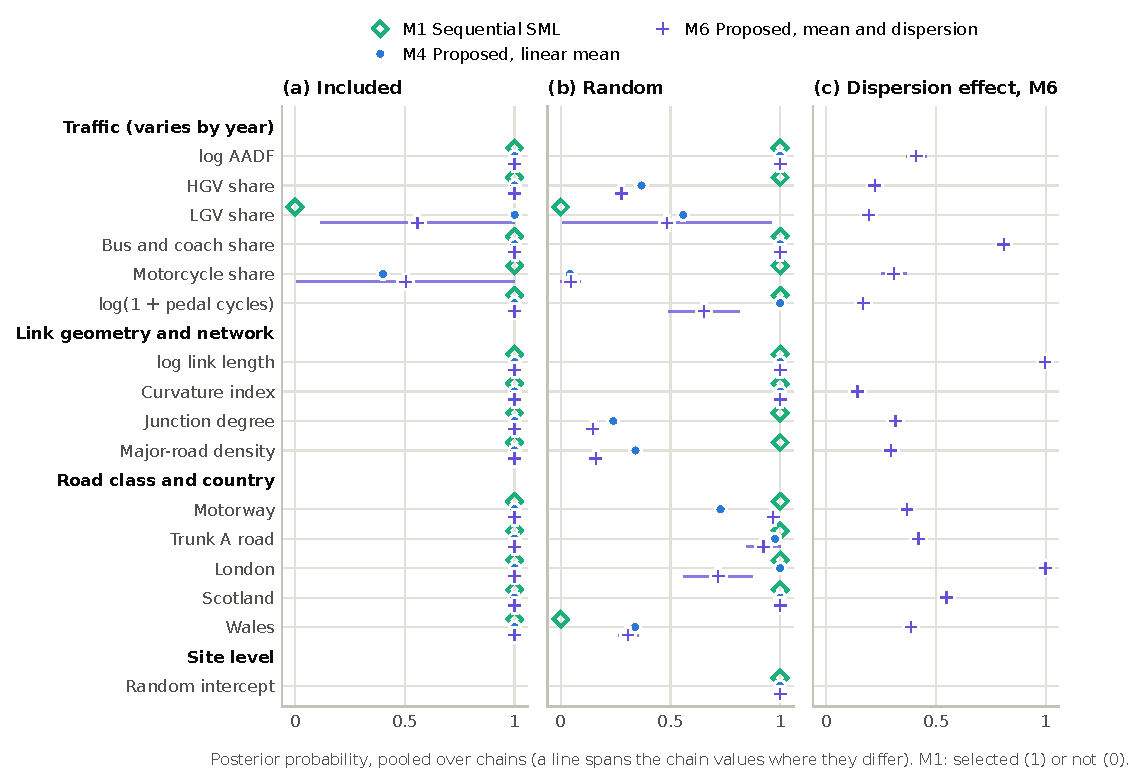
\includegraphics[width=\textwidth]{figures/uk_state_probabilities}
\caption{Specification of the British major-road model. (a) Posterior probability that a candidate is included, fixed or random. (b) Posterior probability that it is random. (c) Posterior probability that it affects the dispersion, under M6. Markers are pooled over chains, and a line spans the chain-specific values where they differ. For M1 the open diamond marks whether the candidate was selected (1) or not (0).}
\label{fig:uk-states}
\end{figure}

\begin{table}[!htbp]
\centering
\begin{threeparttable}
\caption{Model-averaged estimates from M6 for the British major-road links, 2015 to 2018. Continuous candidates are standardized, so coefficients are per standard deviation.}
\label{tab:uk-estimates}
\footnotesize
\setlength{\tabcolsep}{2pt}
\begin{tabular}{@{}lrcccccccc@{}}
\toprule
 & \multicolumn{2}{c}{Mean effect $\beta_j$} & & \multicolumn{2}{c}{Heterogeneity $|\sigma_j|$} & & & \multicolumn{2}{c}{Dispersion $\rho_k$} \\
\cmidrule(lr){2-3}\cmidrule(lr){5-6}\cmidrule(lr){9-10}
Candidate & Mean & 95\% interval & $P_j(\mathrm{R})$ & Mean & 95\% interval & Positive & $P_k(\mathrm{D})$ & Mean & 95\% interval \\
\midrule
\tablerows{tables/uk_estimates_rows.tex}
\bottomrule
\end{tabular}
\begin{tablenotes}\footnotesize
\item $\beta_j$: posterior mean and 95\% interval, averaged over specifications (zero when excluded). $|\sigma_j|$ and Positive (the share of links with a positive coefficient, $\Phi(\beta_j/|\sigma_j|)$) are given when $P_j(\mathrm{R})\ge0.5$, conditional on the parameter being random. $P_k(\mathrm{D})$: posterior probability of a dispersion effect, $\Pr(\eta_k=1\mid\y)$. $\rho_k$ is given when $P_k(\mathrm{D})\ge0.5$, conditional on inclusion. The dispersion is $r_{it}=\exp(\rho_0+\bm w_{it}^\top\bm\rho)$, so a positive $\rho_k$ means less overdispersion.
\end{tablenotes}
\end{threeparttable}
\end{table}

\subsection{Sensitivity}
\tbd{Results under $(a_\sigma,b_\sigma)\in\{(1,1),(1,4)\}$, $\tau_\sigma\in\{0.25,0.5,1\}$, and strong versus weak heredity.}

\section{Discussion}\label{sec:discussion}

\subsection{Extensions}

\paragraph{Heterogeneity in means} Letting the mean of a random parameter depend on site characteristics, $\beta_{ij}=\beta_j+\bm w_i^\top\bm\phi_j+\sigma_j z_{ij}$, adds interaction terms $x_{itj}w_{ik}$ that enter $\psi_{it}$ linearly. They can receive spike-and-slab priors with the heredity constraint $\phi_{jk}\neq0$ only if $\delta_j=1$, and are updated exactly as the $\beta_j$ are.

\paragraph{Correlated random parameters} Writing $\varepsilon_{it}=\x_{it}^\top L\bm z_i$ with $L$ lower triangular, each element $L_{jk}$ enters the linear predictor linearly given $\bm z_i$, so spike-and-slab priors on the off-diagonal elements select correlations in the manner of \citet{fruhwirth2008bayesian}. The collapsed step of Proposition~\ref{prop:marginal} must then integrate over the correlated components jointly. \tbd{Work out whether a rank-one structure keeps this tractable.}

\paragraph{Heterogeneity in variances} A site-dependent standard deviation such as
\[
\sigma_{ij}=\sigma_j\exp(\bm w_i^\top\bm\theta_j)
\]
is no longer linear in $\bm\theta_j$ and requires a Metropolis step, but the selection logic is unchanged.

\paragraph{Other outcomes} Injury severity models with random parameters are logit or ordered models. P\'olya-Gamma augmentation applies directly to binary and multinomial logit likelihoods \citep{polson2013bayesian}, so the three-state prior and the collapsed update carry over.

\paragraph{Scale} For very large networks, the expectation-maximization approach to spike-and-slab selection \citep{rockova2014emvs, rockova2018spike} can locate high-posterior specifications quickly, with the sampler used to quantify uncertainty around them.

\subsection{Limitations}

The random parameters are normal. Heavier-tailed or multimodal heterogeneity, for example finite mixtures \citep{buddhavarapu2016modeling}, would change the variance function in Proposition~\ref{prop:cross} and the integral in Proposition~\ref{prop:marginal}. One-at-a-time indicator updates can mix slowly when candidates are strongly correlated. Most importantly, the method cannot create information that the data do not contain. In cross-sectional data, a selected random parameter remains compatible with covariate-dependent dispersion, and the posterior state probabilities should be read in that light. The method makes this uncertainty visible rather than resolving it.

\section{Conclusions}\label{sec:conclusion}

Random parameters models have changed how unobserved heterogeneity is handled in crash frequency analysis, but the choice of which parameters are random is still made by sequential testing or by searching for a single best specification. This paper replaces that step with a Bayesian model in which each candidate covariate is excluded, fixed or random, and in which the posterior probabilities of these states are estimated jointly with the parameters. The identification results and the simulations explain why random parameters should be interpreted with care in cross-sectional and panel data alike. The sampler makes the approach practical by integrating out the site-specific draws when deciding whether a parameter is random.

In panel data the method recovered the full specification far more often than sequential testing or an information criterion search, and its intervals reflected the uncertainty about which parameters are random. Three practical recommendations follow for agencies developing safety performance functions. First, include squared covariates as fixed-only candidates, because omitted curvature otherwise passes for heterogeneity in cross-sectional and panel data alike. Second, use the false discovery rate rule when the claim of interest is that heterogeneity is present. Third, let the dispersion depend on the candidate covariates and select them in the same model, because a dispersion that varies with a covariate otherwise produces a random parameter on that covariate. In panel data this separates the two explanations. In cross-sectional data it can only divide the posterior between them, and a random parameter selected there should be read as evidence of heterogeneity in either the effect or the dispersion.

The application to 17{,}139 British motorway and A-road links shows these mechanisms in real data. The sequential procedure declared 13 of 15 covariates random. The proposed method declared nine, and modeling the mean curvature and the dispersion changed which effects it found random: two random parameters under a linear mean were explained by curvature, and part of the heterogeneity in another by a covariate-dependent dispersion. The resulting model predicted the next year's collisions better than every alternative. With data of this size almost every candidate is included and most random parameters have probabilities near zero or one, so the value of the method lies less in quantifying uncertainty about a single random parameter than in testing heterogeneity against the alternative explanations that a conventional specification leaves out.


\section*{CRediT authorship contribution statement}
\tbd{Complete per Elsevier CRediT taxonomy.}

\section*{Declaration of competing interest}
The authors declare that they have no known competing financial interests or personal relationships that could have appeared to influence the work reported in this paper.

\section*{Data availability}
\tbd{State data source and access conditions for the application, and the repository for code.}

\appendix
\section{Proofs}\label{app:proofs}

\paragraph{Proof of Proposition~\ref{prop:cross}}
(a) Given $\x_i$, $\varepsilon_i=\sum_j\sigma_jx_{ij}z_{ij}$ is a linear combination of independent standard normal variables, hence normal with mean zero and variance $\sum_j\sigma_j^2x_{ij}^2=v(\x_i)$. Conditional on $\varepsilon_i$, $y_i$ is negative binomial with mean $e^{\eta_i+\varepsilon_i}$ and dispersion $r$. Integrating over $\varepsilon_i$ gives the stated likelihood, which involves $(\sigma_1,\dots,\sigma_p)$ only through $v(\x_i)$.

(b) Let $\lambda_i=e^{\eta_i+\varepsilon_i}$. Since $\E(e^{\varepsilon_i})=e^{v(\x_i)/2}$ and $\E(e^{2\varepsilon_i})=e^{2v(\x_i)}$, we have $\mu_i=\E(\lambda_i)=e^{\eta_i+v(\x_i)/2}$ and $\E(\lambda_i^2)=e^{2\eta_i+2v(\x_i)}=\mu_i^2e^{v(\x_i)}$. By the law of total variance,
\[
\Var(y_i\mid\x_i)=\E(\lambda_i+\lambda_i^2/r)+\Var(\lambda_i)
=\mu_i+\left(1+\tfrac1r\right)\mu_i^2e^{v(\x_i)}-\mu_i^2 ,
\]
which is \eqref{eq:moments}.

(c) Suppose $\sum_jc_jx_j^2=0$ for all $\x$ in the support, for some $c\neq0$. If all $\sigma_j^2>0$, then $\sigma_j^2+tc_j>0$ for all $j$ and all $|t|$ small enough, and the corresponding variance function equals $v(\x)+t\sum_jc_jx_j^2=v(\x)$ on the support. By (a) the likelihood is the same for every such $t$, so the variances are not locally identified. \hfill$\square$

\paragraph{Proof of Corollary~\ref{cor:confounding}}
(i) If $x_j\in\{0,1\}$ then $x_j^2=x_j$, so by \eqref{eq:moments} the log mean is $o_i+\alpha+\sum_{k\neq j}\{\beta_kx_k+\sigma_k^2x_k^2/2\}+x_j(\beta_j+\sigma_j^2/2)$, which depends on $(\beta_j,\sigma_j)$ only through $\beta_j+\sigma_j^2/2$. The variance in \eqref{eq:moments} depends on $v(\x_i)$, which differs by $\sigma_j^2$ between $x_j=1$ and $x_j=0$ with the other covariates held fixed.
(ii) The log mean contains $\beta_jx_j+\sigma_j^2x_j^2/2$, and $\sigma_j^2/2\ge0$.
(iii) An NB model with mean $m$ and dispersion $r(\x)$ has variance $m+m^2/r(\x)$. Taking $m=\mu_i$ and $1/r(\x_i)=(1+1/r)e^{v(\x_i)}-1$, which is positive because $(1+1/r)e^{v(\x_i)}>1$, reproduces both moments in \eqref{eq:moments}. \hfill$\square$

\paragraph{Proof of Proposition~\ref{prop:panel}}
Conditional on the random components, $y_{it}$ and $y_{is}$ are independent with means $\lambda_{it}=e^{\eta_{it}+\varepsilon_{it}}$ and $\lambda_{is}=e^{\eta_{is}+\varepsilon_{is}}$, because the gamma mixing of the negative binomial acts independently in each period. Hence $\Cov(y_{it},y_{is}\mid\cdot)=\Cov(\lambda_{it},\lambda_{is})=\E(\lambda_{it}\lambda_{is})-\mu_{it}\mu_{is}$. The sum $\varepsilon_{it}+\varepsilon_{is}$ is normal with mean zero and variance $v(\x_{it})+v(\x_{is})+2\x_{it}^\top D\x_{is}$, so $\E(\lambda_{it}\lambda_{is})=\exp\{\eta_{it}+\eta_{is}+v(\x_{it})/2+v(\x_{is})/2+\x_{it}^\top D\x_{is}\}=\mu_{it}\mu_{is}\exp(\x_{it}^\top D\x_{is})$. The dispersion $r$ does not appear. \hfill$\square$

\section{Derivation of the conditional updates}\label{app:derivations}

\paragraph{Proposition~\ref{prop:marginal}}
Given the P\'olya-Gamma variables, the working log likelihood is $-\frac12\sum_{i,t}\omega_{it}(\tilde y_{it}-\psi_{it})^2$ up to a constant. Isolating the contribution of $\sigma_jx_{itj}z_{ij}$, the terms that involve $z_{ij}$ for site $i$ are
\[
-\tfrac12\sum_{t}\omega_{it}\left(e_{it}-\sigma x_{itj}z_{ij}\right)^2
=-\tfrac12\sum_t\omega_{it}e_{it}^2+\sigma z_{ij}b_{ij}-\tfrac12\sigma^2z_{ij}^2q_{ij}.
\]
Multiplying by the standard normal density of $z_{ij}$ and integrating,
\begin{align*}
&\int\frac{1}{\sqrt{2\pi}}\exp\left\{-\tfrac12\left(1+\sigma^2q_{ij}\right)z^2+\sigma b_{ij}z\right\}dz\\
&\qquad=\left(1+\sigma^2q_{ij}\right)^{-1/2}\exp\left\{\frac{\sigma^2b_{ij}^2}{2\left(1+\sigma^2q_{ij}\right)}\right\},
\end{align*}
which equals one at $\sigma=0$. Taking the product over sites and logarithms gives \eqref{eq:ell}. Completing the square in the same integrand gives the normal conditional distribution of $z_{ij}$ stated in the proposition.

\paragraph{Fixed effects}
The terms of the working log likelihood that involve $\beta_j$ are $B_j\beta_j-\frac12S_j\beta_j^2$ up to a constant. Integrating against the $\Normal(0,\tau_\beta^2)$ slab gives
$\tau_\beta^{-1}(S_j+\tau_\beta^{-2})^{-1/2}\exp\{B_j^2/(2(S_j+\tau_\beta^{-2}))\}$, which equals \eqref{eq:bf-beta}, and the conditional distribution of $\beta_j$ given $\gamma_j=1$ is normal with precision $S_j+\tau_\beta^{-2}$ and mean $B_j/(S_j+\tau_\beta^{-2})$.

\paragraph{Dispersion}
With $p_{it}=e^{\psi_{it}}/(1+e^{\psi_{it}})$, the negative binomial probability is proportional to $\{\Gamma(y_{it}+r)/\Gamma(r)\}(1-p_{it})^r$ as a function of $r$. Since $\Gamma(y+r)/\Gamma(r)=\sum_{l=0}^{y}|s(y,l)|\,r^l$, with $|s(y,l)|$ unsigned Stirling numbers of the first kind, introducing $L_{it}$ with $\Pr(L_{it}=l\mid y_{it},r)\propto|s(y_{it},l)|r^l$, which is the $\CRT(y_{it},r)$ distribution, gives a joint density proportional to $r^{\sum L_{it}}\exp\{-r\sum\log(1+e^{\psi_{it}})\}$. With a $\Gammad(a_r,b_r)$ prior the full conditional of $r$ is $\Gammad\left(a_r+\sum L_{it},\ b_r+\sum\log(1+e^{\psi_{it}})\right)$ \citep{zhou2015negative}.


\bibliographystyle{elsarticle-harv}
\bibliography{references}

\end{document}
